\section{Aufgabe der Komponente}
Die Broadcast Komponente ermöglicht es den Benutzern von SharkNet, Nachrichten an andere Benutzer zu schicken. Dabei können auch andere Komponenten, wie etwa der semantische Eingans- und Ausgangsfilter zum Einsatz kommen, was jedoch nicht zwingend erforderlich ist. Falls auf einen Eingangsfilter oder Ausgangsfilter verzichtet werden sollte, werden wie bei einem klassischen Broadcast die Nachrichten an alle sich in der Nähe befindlichen Geräte versendet. Inwiefern der klassische Broadcast vom Benutzer semantisch eingeschränkt werden kann, lässt sich in der Komponentenbeschreibung der Komponente Semantischer Filter in Erfahrung bringen.

\section{Architektur}

\subsection{Überlick}\label{ch:broadcastcomps}
Die folgenden Komponenten werden von der Komponente Broadcast zwingend benötigt:
\begin{itemize}
\item WifI 
\item Bluetooth 
\item Persistenz 
\end{itemize}
Optional sind hingegen die Komponenten:
\begin{itemize}
	\item Semantischer Filter
\end{itemize}

\subsection{Überlick}\label{ch:broadcastoverview}
Die Komponente bildet sich vorrangig aus sieben Klassen, wovon drei sich innerhalb des SharkFrameworks und vier sich innerhalb der App befinden. Diese sieben Klassen werden nun ausgehend von der folgenden Abbildung kurz beschrieben.
\begin{figure}[H]
	\centering
	\hspace*{1cm}
	\makebox[\linewidth][c]{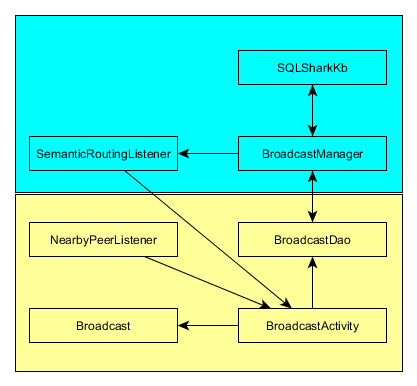
\includegraphics[width=0.9\linewidth]{general/BroadcastStruktur1.png}}%
	\caption{Die Klassen der Broadcast Komponente}
	\label{fig:broadcastStructure}
\end{figure}
\begin{itemize}
	\item Die SQLSharkKb ist eine Implementierung der Shark Knowledgebase mit SQLite. Mit ihr werden sämtliche Daten wie bsp. die Nachrichten, semnatische Annotationen oder auch Benutzerprofile gespeichert. Sie nimmt ausschließlich Anfragen von Klassen aus dem SharkFramework entgegen.
	\item Der BroadcastManager ist die direkte Schnittstelle zwischen dem Framework und der App. Er nimmt Broadcast-Objekte vom BroadcastDao entgegen und lässt diese gegebenfalls von der SQLSharkKb speichern. Sollte eine neue Nachricht den Peer erreichen, wird vom BroadcastManager die Nachricht auf ihre semantische Relevanz hin überprüft und im Erfolgsfall der Wissenbasis des Peers hinzugefügt.
	\item Der SemanticRoutingListener liefert neue vom BroadcastManager akzeptierte Nachrichten an die BroadcastActivity
	\item Der BroadcastDao nimmmt von der BroadcastActivity veränderte Nachrichten in Form eines Objekts vom Typ Broadcast entgegen, baut diese in für das SharkFramework vewertbare Objekte vom Typ ASIPSpace um und leitet diese an den BroadcastManager weiter.
	\item Wann immer die Anzahl der sich in Reichweite befindlichen Peers ändert, wird die BroadcastActivity vom NearbyPeerListener mit einer angepassten Liste von Peers versorgt.
	\item Die BroadcastActivity ist die Schnittstelle zwischen Benutzer und App. Sie nimmt neue Nachrichten vom Benutzer entgegen, wobei das Hinzufügen von semantischen Annotationen optional ist. Sie benutzt die Entitätsklasse Broadcast um die Nachrichten in einer Klasse zu bündeln, welche bei Aktualisierungen an das BroadcastDao weitergereicht wird. 
\end{itemize}

\subsection{Schnittstellendefinitionen}\label{ch:broadcastinterfaces}


\section{Nutzung}
Die Komponente ist in der App innerhalb der \textit{BroadcastActivity} eingebunden. Der Endanwender kann über die diese Activity und die dazugehörige XML-Datei die Nachrichten versenden, betrachten und mit semantischen Annotationen versehen, wobei Letzteres auch die Komponente Semantische Filter betrifft.
\\Die Komponente kann aber auch in eigenen Activities benutzt werden ohne die vorgegebene \textit{BroadcastActivity} benutzen zu müssen. Der Entwickler muss bei seiner eigenen Activity dafür lediglich von der Klasse \textit{BaseActivity} erben. Die Klasse \textit{BaseActivity} stellt das Attribut \textit{mApi} vom Typ \textit{SharkNetApi} bereit, mit dem durch die Methoden \textit{getBroadcast()} und \textit{updateBoradcast(...)} der Broadcast geliefert und verändert werden kann.
\\

\subsection{Code}
Der Code dieser Komponente kann hier \url{https://github.com/SharedKnowledge/SharkNet/tree/master/app/src/main/java/net/sharksystem/sharknet} betrachtet werden. 

\subsection{Deployment / Runtime}
...


\section{Test}



\section{Ausblick}
Der Austausch von Nachrichten mit mehreren Geräten in der Nähe funktioniert grundlegend sicher, aber noch nicht komplett fehlerlos. So kann es bei hoher Last seitens der Benutzer passieren, dass einige Nachrichten nicht empfangen werden können, obwohl sie gemäß dem eingestellten semantischen Filter akzeptiert werden müssten. 